\section{Ergebnisse}
\label{sec:ergebnisse}
\subsection{Versuchteil 1:}
 
 \begin{itemize}
 	\item Interpretation mit Reaktionsgleichung Sauerstoff\\
 		\begin{flalign}\label{gl:5}
 			\ce{O2 + 2 e^- + 2 H2O -> H2O2 + 2 OH-}
 		\end{flalign}
 		\begin{flalign}\label{gl:6}
 		\ce{H2O2 + 2 e^- -> 2 OH^-}
 		\end{flalign}
 	\item Vergleich Polarogramm geglättet und ungeglättet\\
 	Das ungeglättete Polarogramm (vgl. Abb.\ref{fig:daten_farbig} in gelb) zeigt den Stomstärkeverlauf in Anwesenheit von Sauerstoff. Es treten Peaks auf, wenn die Reduktionsreaktionen (\ref{gl:5}) bei etwa \SI{0}{\volt} und (\ref{gl:6}) bei etwa \SI{-1}{\volt} ablaufen. Nach erfolgter Spülung mit Stickstoff ist der Sauertoff aus der Lösung verschwunden. Er kann nicht mehr reduziert werden und stört darum auch nicht mehr das Polarogramm (vgl. Abb.\ref{fig:daten_farbig} in schwarz) welches damit als geglättet anzusehen ist. Es besitzt nun einen quasi horizontalen Verlauf.
 	
 	\item Zuordnung Begründen\\
 Die Peaks können den enthaltenen Elementen aufgrund ihrer Stellung in der elektrochemischen Spannungsreihe zugeordnet werden. Je edler ein Metall ist, umso höher ist auch das entsprechende Standardelektrodenpotential und umso eher wird es reduziert. \\
 Dder zweite Peak kann besonders sicher dem Blei zugeordnet werden, da durch wissentliche Erhöhung der Bleikonzentration ein größerer Ausschlag erkennbar ist.
 \end{itemize}
 
 %Start
 \begin{figure}[h!]
 	\centering
 	\includegraphics[width=0.9\textwidth]{img/Daten_farbig2}
 	\caption{Strom-Spannungskurven (Polarogramme) des Versuchsteils 1}
 	\label{fig:daten_farbig}
 \end{figure}
 \FloatBarrier
 %Ende     
 %Tabelle START
 \vspace*{-2.5mm}
 \renewcommand{\arraystretch}{1.2}
 \begin{table}[h!]
 	\centering
 	\caption{Zuordnung der Peaks den Elementen des Multielementencocktails}
 	\label{tab:peaks}
 %	\resizebox{17cm}{!}{
 	\begin{tabulary}{\textwidth}{|C|C|C|C|C|}
 		\hline
 		\textbf{Element} &  \textbf{Kupfer}  &\textbf{Blei}& \textbf{Cadmium} & \textbf{Zink}\\ 
 	&\ce{Cu}&\ce{Pb}&\ce{Cd}&\ce{Zn}\\
 		\hline
 		\textbf{Peak} &1&2&3&4\\
 		\hline
 		\textbf{Std.-Elektrodenpotential [V]}&$+0,52$&$-0,13$&$-0,40$&$-0,76$\\
 		\hline
 	\end{tabulary}
 	%}
 \end{table}
 \FloatBarrier
 \vspace*{-2.5mm}
 %Tabelle ENDE
 
 
\newpage
 
 \subsection{Versuchsteil 2:}

\begin{itemize}
	\item  Polarogramm Probe mit Aufstockungen ?
	\item  Quantitative Auswertung des Programms
	\item  MANUELLE KALIBRIERGERADE !!\\
	Die Kalibriergerade wird manuell erstellt in dem die die gemessenen Stromstärken der Peaks über dem Konzentrationszuschuss durch die Zugabe der Blei Standardlösung aufgetragen werden. Die Stromstärken für die Y-Achse werden aus den gewonnenen Polarogrammen abgelesen. Hier treten Ablesefehler von etwa $\pm$ \SI{10}{\nano\ampere} auf. Die Konzentrationsänderung bei Addition von Standardlösung wird entsprechend der Gleichungen \ref{gl:7} und (\ref{gl:8}) berechnet. 
	
	\begin{figure}[h!]
		\begin{center}
			\resizebox{0.8\textwidth}{!}{
				\begin{tikzpicture}[trim axis left, trim axis right]
				\begin{axis}[
				axis lines = left,
				width = 13cm,
				height = 7cm,
				xmin = 0,
				xmax = 17,
				ymin = 0,
				ymax = 450,
				%ytick = {0,2,...,14},
				%xtick = {0,10,...,100},
				ylabel={c(NaOH) in [\si{\milli\mole\per\liter}]},
				xlabel={t in [\si{\second}]},
				%	legend style={at={(0.5,0.95)},anchor=west}
				]
				
\addplot[scatter,only marks,
scatter src=explicit symbolic]
coordinates {
	(8,100)  [a]
	(10,100) [c]
	(0.02,0.17) [a]
	(0.06,0.1)  [a]
	(0.9,0.5)   [b]
	(0.5,0.3)   [c]
	(0.85,0.52) [b]
	(0.12,0.05) [a]
	(0.73,0.45) [b]
	(0.53,0.25) [c]
	(0.76,0.5)  [b]
	(0.55,0.32) [c]
};
				\end{axis}
				\end{tikzpicture}
			}
			\caption{Konzentration von NaOH über der Zeit}
			\label{dia:c/t}
		\end{center}
	\end{figure}
	\FloatBarrier
	\item  Aliquotierfaktor\\
\end{itemize}

\textbf{Berechnung der Blei-Standard-Zugaben-Konzentration:}
\begin{flalign}\label{gl:7}
	V_{\text{Standard-Zugabe}} * c_{\text{Standard-Zugabe}} &= V_{\text{Lösung}} * c_{\text{Lösung}}\\
	c_{\text{Lösung}} 	&= \frac{V_{\text{Standard-Zugabe}} }{V_{\text{Lösung}}} * c_{\text{Standard-Zugabe}}		
\end{flalign}
\begin{flalign}\label{gl:8}
	c_{\text{Lösung},1} &=\frac{\SI{200e-6}{\liter}}{\SI{25e-3}{\liter}} * \SI{1000}{\milli \gram \per \liter}\\
	&= \underline{\SI{8}{\milli \gram \per \liter}	}\\[3mm]
	c_{\text{Lösung},2} &=\frac{\SI{400e-6}{\liter}}{\SI{25e-3}{\liter}} * \SI{1000}{\milli \gram \per \liter}\\
	&= \underline{\SI{16}{\milli \gram \per \liter}	}
\end{flalign}

 %Tabelle START
\vspace*{-2.5mm}
\renewcommand{\arraystretch}{1.2}
\begin{table}[h!]
	\centering
	\caption{Messreihe 1 mit berechneten Leistungen}
	\label{tab:messreihe1}
	%\resizebox{10cm}{!}{
	\begin{tabulary}{\textwidth}{C|CCC}
		\hline
		\textbf{Konzentration der Bleizugabe in \si{\milli \gram \per \liter}} &  \textbf{Spannung in \si{\volt}}  &\textbf{Stromstärke in \si{\nano \ampere}}& \textbf{Leistung in \si{\nano \watt}}\\ 
		\hline
		0 	&-0,376	&-113,0	&42,488\\
		0 	&-0,376	&-112,5	&42,300\\
		8 	&-0,376	&-268,2	&100,843\\
		8 	&-0,376	&-266,6	&100,242\\
		16 	&-0,376	&-422,8	&158,973\\
		16 	&-0,382	&-416,0	&158,912\\
		\hline
	\end{tabulary}
	%}
\end{table}
\FloatBarrier
\vspace*{-2.5mm}
%Tabelle ENDE
 %Tabelle START
\vspace*{-2.5mm}
\renewcommand{\arraystretch}{1.2}
\begin{table}[h!]
	\centering
	\caption{Messreihe 2 mit berechneten Leistungen}
	\label{tab:messreihe2}
	%\resizebox{10cm}{!}{
	\begin{tabulary}{\textwidth}{C|CCC}
		\hline
		\textbf{Konzentration der Bleizugabe in \si{\milli \gram \per \liter}} &  \textbf{Spannung in \si{\volt}}  &\textbf{Stromstärke in \si{\nano \ampere}}& \textbf{Leistung in \si{\nano \watt}}\\ 
		\hline
		0 	&-0,382	&-129,3	&49,393\\
		0 	&-0,382	&-139,2	&53,174\\
		8 	&-0,382	&-286,2	&109,328\\
		8 	&-0,382	&-282,2	&107,800\\
		16 	&-0,382	&-425,1	&162,388\\
		16 	&-0,382	&-424,0	&161,968\\
		\hline
	\end{tabulary}
	%}
\end{table}
\FloatBarrier
\vspace*{-2.5mm}
%Tabelle ENDE

%\begin{figure}[h!]
%	\begin{center}
%		\resizebox{0.95\textwidth}{!}{
%		\begin{tikzpicture}[trim axis left, trim axis right]
%		\begin{axis}[
%		axis lines = middle,
%		width = 20cm,
%		height = 10cm,
%		xmin = -10,
%		xmax = 20,
%	%	ymin = -0.1,
%	%	ymax = 0,
%	%	ytick = {-4.5,-4,...,-1},
%	%	xtick = {-10,-9,...,20},
%		ylabel={Leistung in \si{\nano \watt}},
%		y label style={at={(0.25,0.40)}, rotate=90},
%		xlabel={Konzentration der Blei-Standard-Zugabe in \si{\milli \gram \per \milli \liter}},
%		legend style={at={(0.75,0.45)},anchor=west}
%		]
%		\addplot table {datenm1.dat};
%		\addplot +[mark=none, dashed, black, domain=-10:20] {-2e-8*x-1e-7};
%		\addplot table {datenm2.dat};
%		\addplot +[mark=none, dotted, black, domain=-10:20] {-2e-5*x - 0.0001};
%		
%		\legend{Messreihe 1, Regression Messreihe 1,Messreihe 2, Regression Messreihe 2};
%		\end{axis}
%		\end{tikzpicture}
%			}
%		\caption{Berechnete Leitungen in Abhängigkeit von der Konzentration der Blei-Standardzugabe (siehe Tab. \ref{tab:messreihe1} und Tab. \ref{tab:messreihe2})}
%		\label{dia:lnr/lnc}
%	\end{center}
%\end{figure}
%\FloatBarrier
%\vspace*{-5mm}

\pagebreak

 \includepdf[pages=2-5]{Daten_farbig2}